\documentclass[11pt]{standalone}
\usepackage{amssymb}
\usepackage{amsmath}
\usepackage[no-math]{fontspec}
\usepackage{unicode-math}
\usepackage{libertinus}
\usepackage{pgf,xcolor}
\usepackage{tikz}
\usetikzlibrary{arrows.meta, backgrounds}
\usepackage{pgfplots}
\pgfplotsset{compat=newest}

\definecolor{my_darkgray}{HTML}{484949}
\definecolor{my_lightgray}{HTML}{F3F4F4}
\definecolor{my_darkblue}{HTML}{005A94}
\definecolor{my_lightblue}{HTML}{CCDEE9}
\definecolor{my_yellow}{HTML}{FFEC7F}
\definecolor{my_red}{HTML}{E60000}
\definecolor{my_orange}{HTML}{E87846}

\begin{document}
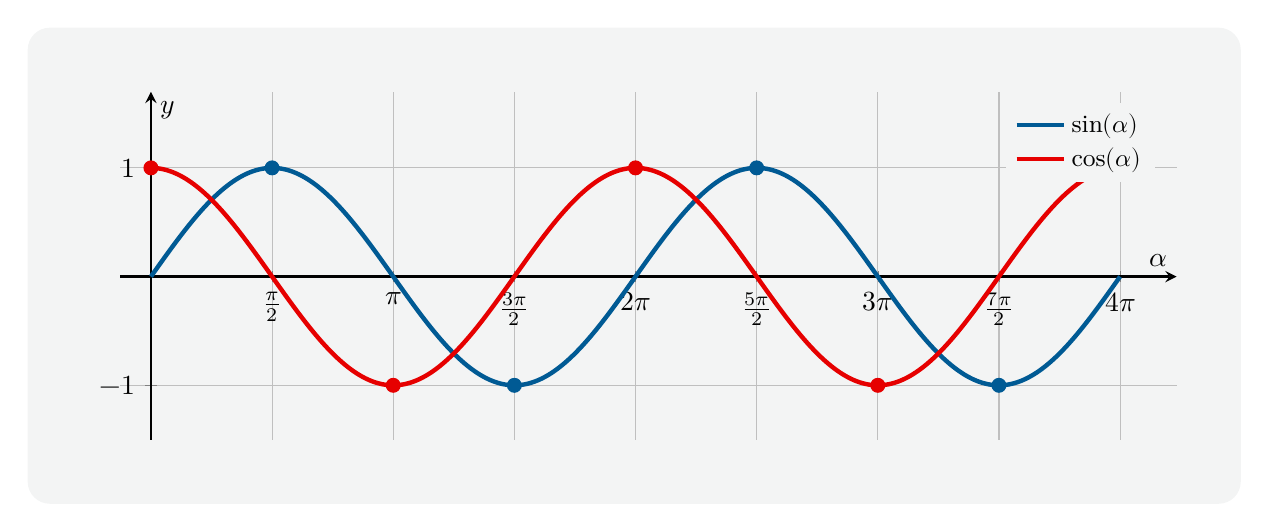
\begin{tikzpicture}[
    show background rectangle,
    background rectangle/.style={fill=my_lightgray, rounded corners=8pt},
    inner frame sep=0.8cm
]
\begin{axis}[
    axis lines=center,
    xlabel={$\alpha$},
    ylabel={$y$},
    height=6cm, width=15cm,
    xmin=-0.4, xmax=13.3,   % slightly beyond 4pi ~ 12.57
    ymin=-1.5, ymax=1.7,
    % x-axis ticks at multiples of pi/2
    xtick={
        0,
        1.5708, 3.1416, 4.7124, 6.2832,
        7.8540, 9.4248, 10.9956, 12.5664
    },
    xticklabels={
        $0$,
        $\frac{\pi}{2}$, $\pi$, $\frac{3\pi}{2}$, $2\pi$,
        $\frac{5\pi}{2}$, $3\pi$, $\frac{7\pi}{2}$, $4\pi$
    },
    ytick={-1, 0, 1},
    grid=both,
    axis line style={thick},
    legend style={
        font=\small,
        at={(0.98, 0.97)},
        anchor=north east,
        draw=none,
        fill=my_lightgray,
    },
    legend cell align=left,
    clip=true,
]

% sin(alpha): my_darkblue
\addplot[draw=my_darkblue, samples=500, ultra thick, domain=0:4*pi]
    {sin(deg(x))};
\addlegendentry{$\sin(\alpha)$}

% cos(alpha): my_red
\addplot[draw=my_red, samples=500, ultra thick, domain=0:4*pi]
    {cos(deg(x))};
\addlegendentry{$\cos(\alpha)$}

% Mark key maxima and minima for sine
% sin maxima at pi/2 and 5pi/2; minima at 3pi/2 and 7pi/2
\addplot[only marks, mark=*, mark size=2.5pt, draw=my_darkblue, fill=my_darkblue]
    coordinates{
        (1.5708,  1)    % pi/2
        (7.8540,  1)    % 5pi/2
        (4.7124, -1)    % 3pi/2
        (10.9956,-1)    % 7pi/2
    };

% Mark key maxima and minima for cosine
% cos maxima at 0 and 2pi and 4pi; minima at pi and 3pi
\addplot[only marks, mark=*, mark size=2.5pt, draw=my_red, fill=my_red]
    coordinates{
        (0,       1)
        (6.2832,  1)    % 2pi
        (12.5664, 1)    % 4pi
        (3.1416, -1)    % pi
        (9.4248, -1)    % 3pi
    };

\end{axis}
\end{tikzpicture}
\end{document}
